\mode<article>
Siguiendo el método de las diferencias Finitas, 
sólo resta reemplazar las ecuaciones \ref{EqEcuacionDerivadaX} 
y \ref{EqEcuacionDerivadaY} en la \ref{EqEcuacionPoisson}. Puede
verse fácilmente\footnote{hágalo, ¡atrévase!} que \emph{para el 
conjunto de nodos del interior de la chapa } se puede escribir
la ecuación

\begin{equation}\label{EqEcuacionDiferenciasFinitas}
  \begin{aligned}
    \frac{T_{k+1} - 2T_k +T_{k-1} }
    {\Delta x ^2}    
    +
    \frac{T_{k+N_x} - 2T_k +T_{k-N_y} }
    {\Delta y ^2}
    &= 0 \\
    \beta ^2 T_{k-N_x}+T_{k-1} 
    - 2\big(1+\beta^2\big) T_k
    +T_{k+1} + \beta^2 T_{k+N_x} &= 0
  \end{aligned}
\end{equation}

donde se ha definido 
\begin{equation}\label{EqEcuacionBeta}
  \beta = \frac{\Delta x}{\Delta y}
\end{equation}

La ecuación 
\ref{EqEcuacionDiferenciasFinitas}
es válida para todos los nodos de índice
$k$ tal que siguiendo la biyección de la
ecuación \ref{EqEcuacionRelacionIndices}
se tiene que $0<i<N_x$ y $0<j<N_y$, donde
el uso del menor estricto refleja que
los nodos no estan en los bordes. 
Para los
nodos de los bordes debemos tomar una 
consideración especial. 

Aún en este caso general, podemos ver 
lo siguiente. Cada nodo interno de la chapa
cumple la ecuación \ref{EqEcuacionDiferenciasFinitas}. Si las 
temperaturas de los nodos están dispuestas en
el vector $\vec{T}$ de la ecuación \ref{EqEcuacionVectorT}
la ecuación diferencial surge de multiplicar
un vector fila por el vector columna $\vec{T}$.
El conjunto de ecuaciones para todos los $k$
internos genera entonces un sistema lineal 
cuyos coeficientes están bien determinados 
en la ecuación \ref{EqEcuacionDiferenciasFinitas},
como se muestra en la Figura \ref{FiguraCoeficientesMatriz}.

\begin{figure}
  \includeslide[width=\textwidth]{FrameCoeficientesMatriz}
  \caption{Ilustración de la construcción de los coeficientes de matríz
  para la fila $k$-ésima de la matriz del sistema lineal, para algún
  $k$ correspondiente a un nodo del interior de la chapa.
  \label{FiguraCoeficientesMatriz}}

\end{figure}
\mode*

\begin{frame}<presentation>[label=FrameEciacionInterior]
  \frametitle{Matricialización de la Ecuación Diferencial}
 $$\beta ^2 T_{k-N_x}+T_{k-1}- 2\big(1+\beta^2\big) T_k +T_{k+1} + \beta^2 T_{k+N_x} = 0$$

  \begin{columns}
    \column{0.6\textwidth}
    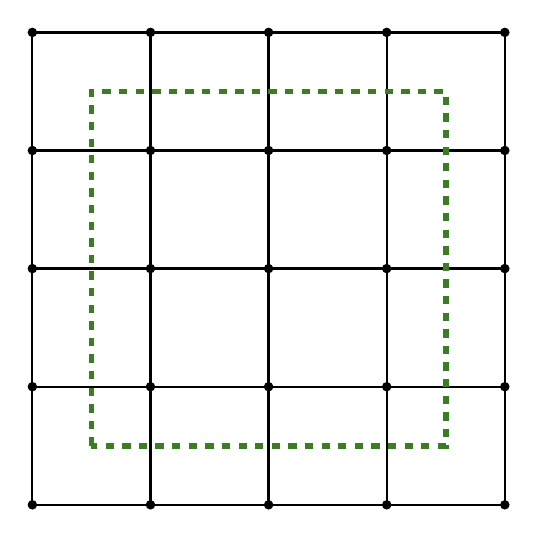
\begin{tikzpicture}[scale=1.5]
      \draw [thick] (-2,-2) grid (2,2) ;
      \foreach \x in {-2,-1,0,1,2}
        \foreach \y in {-2,-1,0,1,2}
	{
	  \draw [fill=black] (\x,\y) circle (1pt);
	  };
      \draw [dashed,OliveGreen,line width=2pt] (-1.5,-1.5) rectangle (1.5,1.5);
    \end{tikzpicture}

    \column{0.4\textwidth}
    %\begin{equation}
      \resizebox{2cm}{!}{$\big[\mathbf{M}\big] $}
$  \begin{pmatrix}
    T_1 \\ T_2 \\ \vdots \\ T_{Nx Ny}
  \end{pmatrix} 
  =  \vec{b} $
% \end{equation}
  \end{columns}

\end{frame}

\begin{frame}<presentation>[label=FrameCoeficientesMatriz]
  \frametitle{Coeficientes de Matriz}
  \centering
%  \framesubtitle{Para los nodos internos}
  \tikz [baseline] \node  (ecuacion) at (0,0)  {
    $\beta ^2 T_{k-N_x}+T_{k-1}- 
    2\big(1+\beta^2\big) T_k +T_{k+1} + \beta^2 T_{k+N_x} = 0$
  };

  \vspace{0.5cm}

\flushleft
  Fila $k$-esima: 

\centering

  \vspace{0.5cm}

  $M [k,:] = \Big[ \dotsi $ 
  \tikz[baseline] \node [anchor=base] (-b2) at (0,0) {$\beta^2$} ;
  $ \dotsi $
  \tikz[baseline] \node [anchor=base] (k-1) at (0,0) {$1$};
  $ \dotsi  $
  \tikz[baseline] \node [anchor=base] (diag) at (0,0) {$-2\big(1+\beta^2\big)$};
  $ \dotsi $
  \tikz[baseline] \node [anchor=base] (k+1) at (0,0) {$1$};
  $\dotsi $  
  \tikz[baseline] \node [anchor=base] (b2) at (0,0) {$ \beta^2$} ;
  $ \dotsi \Big]$
  \tikz[overlay,->] \draw [blue] (-b2.south west) -- ($(-b2)-(2,2)$)  node[text=black,anchor=north] {$k-N_x$};
  \tikz[overlay,->] \draw [blue] (k-1.south)      -- ($(k-1)-(1,2)$)  node[text=black,anchor=north] {$k-1$};
  \tikz[overlay,->] \draw [blue] (diag.south)     -- ($(diag)-(0,2)$) node[text=black,anchor=north] {$k$};
  \tikz[overlay,->] \draw [blue] (k+1.south)      -- ($(k+1)-(-1,2)$) node[text=black,anchor=north] {$k+1$};
  \tikz[overlay,->] \draw [blue] (b2.south)       -- ($(b2)-(-2,2)$)  node[text=black,anchor=north] {$k+N_x$};

  \vspace{3cm}

  \hfill  \tikz[baseline]  \node (b0) at (-0.5,0) {$b_k  = 0$}; 
  \hspace{1cm} \tikz[baseline,fill=none]  \node (help) at (0,0) {};
  \tikz[overlay] \draw [->,>=latex,blue] (ecuacion.east) -| (help.west) -- (b0.east);
 
\end{frame}

\mode<all>
